\documentclass[11pt]{article}
\usepackage[left=25mm,right=25mm,top=30mm,bottom=30mm]{geometry}

\usepackage{indentfirst}
\setlength\parindent{1.0em}
%한글 문서이므로 첫 줄 들여쓰기 적용, 너비는 1 전각 문자 크기로 조정

\usepackage{amsmath} % math
\usepackage{amssymb} % math
\usepackage{graphicx} % to use \includegraphics{}
\usepackage{diagbox} % to make advanced tables
\usepackage{multirow} % to make advanced tables 

\usepackage[nonfrench,hangul]{kotex} % to use Korean
\usepackage{dhucs-setspace}
\SetHangulspace{1.5}{1.2}
\usepackage[ensec]{dhucs-sectsty}
%한글 사용 관련 패키지
%본문 줄 간격 150 %, 표 줄 간격 120 %
%제 # 절 표현이 거추장스러우므로 제거

\usepackage{color} % to use color font 
\usepackage{hyperref} % to insert hyperlinks

\makeatletter
\newcommand{\website}[1]{%
	\newcommand{\@website}{#1}%	
}
\renewcommand{\maketitle}{%
	\newpage
	\begin{center}%
		{\LARGE \@title \par}%
		\vskip 0.5em%
		{%
			\normalsize
			\begin{tabular}[t]{c}
				마지막 수정일 : \@date \\
				공식 웹사이트 : \@website
			\end{tabular}
		}
	\end{center}
}
\makeatother
%제목 형식

\newcommand*\kotex{%
	\texorpdfstring{%
		\textsf{k}\kern-0.0625em%
		\textit{o}\kern-1.5pt\lower.15ex%
		\hbox{.}\kern-1pt\protect\TeX%
	}{ko.TeX}%
}
%kotex 글자 모양 정의

\newcommand{\lshort}{%
	\href{http://texdoc.net/texmf-dist/doc/latex/%
		lshort-korean/lshort-kr.pdf%
	}{\LaTeXe 입문}%
}
%입문서 번역본 파일 링크

\usepackage{etoolbox}
\usepackage[svgnames]{xcolor}
\usepackage{tikz}
\usepackage{framed}
\usepackage[utf8]{inputenc}
\usepackage[T1]{fontenc}
\usepackage{libertine} % or any other font package
\newcommand*\quotefont{\fontfamily{LinuxLibertineT-LF}} % selects Libertine as 
%the quote font

\newcommand*\quotesize{60} % if quote size changes, need a way to make shifts 
%relative
% Make commands for the quotes
\newcommand*{\openquote}
{\tikz[remember picture,overlay,xshift=-4ex,yshift=-2.5ex]
	\node (OQ) 
	{\quotefont\fontsize{\quotesize}{\quotesize}\selectfont``};\kern0pt}

\newcommand*{\closequote}[1]
{\tikz[remember picture,overlay,xshift=4ex,yshift={#1}]
	\node (CQ) {\quotefont\fontsize{\quotesize}{\quotesize}\selectfont''};}

% select a colour for the shading
\colorlet{shadecolor}{Azure}

\newcommand*\shadedauthorformat{\emph} % define format for the author argument

% Now a command to allow left, right and centre alignment of the author
\newcommand*\authoralign[1]{%
	\if#1l
	\def\authorfill{}\def\quotefill{\hfill}
	\else
	\if#1r
	\def\authorfill{\hfill}\def\quotefill{}
	\else
	\if#1c
	\gdef\authorfill{\hfill}\def\quotefill{\hfill}
	\else\typeout{Invalid option}
	\fi
	\fi
	\fi}
% wrap everything in its own environment which takes one argument (author) and 
%one optional argument
% specifying the alignment [l, r or c]
%
\newenvironment{shadequote}[2][l]%
{\authoralign{#1}
	\ifblank{#2}
	{\def\shadequoteauthor{}\def\yshift{-2ex}\def\quotefill{\hfill}}
	{\def\shadequoteauthor{%
		\par\authorfill\shadedauthorformat{#2}%
	}\def\yshift{2ex}}
	\begin{snugshade}\begin{quote}\openquote}
		{\shadequoteauthor\quotefill\closequote{\yshift}\end{quote}%
	\end{snugshade}
}
%이상 shadequote 정의

\begin{document}

\title{An Introduction to \LaTeX\enspace ver 1.9}
\date{2016년 2월 7일}
\website{http://gshslatexintro.github.io/gshslatexintro}
\maketitle

\section{기초}

\subsection{\LaTeX 이란?}
\LaTeX 은 문서의 모습을 보면서 작업하는 한/글이나 Microsoft Word와는 달리, 
TeXeditor를 통해 문서 코드를 작성하고, 컴파일하여 pdf 문서를 생성해어 문서를 
작성하는 프로그램이다.

처음 사용법을 배울 때에는 어려울 수 있지만 익숙해진다면 미려한 조판의 문서를 
쉽게 얻을 수 있는 매우 편리한 도구이다.

\subsection{설치하기}

\subsubsection{TeXLive(+\kotex)}
TeX를 사용하기 위해서는 먼저 TeXLive를 설치해야 한다. 설치는 다음 
링크(ktug)에 접속하여 권장 설치 방법을 따라 진행하면 된다.
\url{http://www.ktug.org/xe/?mid=install}

ktug에서 배포하는 TeXLive는 2014년 이후 판부터 \kotex 를 같이 제공하므로 한 
번에 설치할 수 있다.

용량이 매우 크고 오래 걸리는 작업이므로 안정적인 인터넷 환경에서 시간적 여유를 
가지고 설치하시는 것이 좋다.

\subsubsection{TeX 편집기}
TeX을 사용하려면 TeX 편집기(TeXeditor)가 있어야 한다. 위의 TeXLive를 설치했다면 
기본적으로 TeXworks라는 편집기가 같이 설치된다.
TeX 편집기는 Texmaker, TeXworks, TeXstudio 등등 여러 종류가 
있다.\footnote{Eclipse 사용자의 경우 내장된 TeXclipse plugin이 있다고 하지만 
여기서는 설명하지 않는다. 더 많은 TeX 편집기의 목록은
\href{https://en.wikipedia.org/wiki/Comparison_of_TeX_editors}{\textbf{여기}} 
에 있으나 입문자에게는 딱히 필요없다.}

기본적으로 설치되는 TeXworks를 사용하여도 좋으나 더 많은 기능이 있는 
TeXstudio를 추가로 설치하여 사용하기를 권한다. 
\url{http://www.texstudio.org/}를 통해 설치할 수 있으며 Linux, Mac, Windows 
환경에서 사용할 수 있다.

참고로 TeXstudio에서 한글 글꼴이 포함되지 않은 고정폭 글꼴을 사용할 경우, 그림 
\ref{texstudio}처럼 한글이 전부 굴림으로 표시된다. 이는 단순히 글꼴이 보기 좋지 
않음의 문제를 넘어, 한글과 영어의 폭이 맞지 않는다는 문제가 있다.
네이버 개발자센터에서 배포하는 '나눔고딕코딩' 폰트나 'D2Coding' 폰트를 이용하면 
이러한 문제를 해결할 수 있다. 나눔고딕코딩은 현재 지원이 끊긴 폰트이므로 
D2Coding을 이용하는 것을 추천한다.
\href{http://dev.naver.com/projects/d2coding}{D2Coding 다운로드 링크}
폰트를 다운받아 설치한 뒤 TeXstudio의 Options-Configure TeXstudio-Editor-Font 
Family에서 D2Coding으로 설정하면 된다.

온라인 TeX 편집기도 있다. 특히 \href{https://www.sharelatex.com/}{ShareLaTeX} 와 같은 온라인 TeX 편집기의 경우 Google Docs처럼 tex문서를 동시에 편집할 수 있어서 유용하다.

\begin{figure}
	\begin{center}
		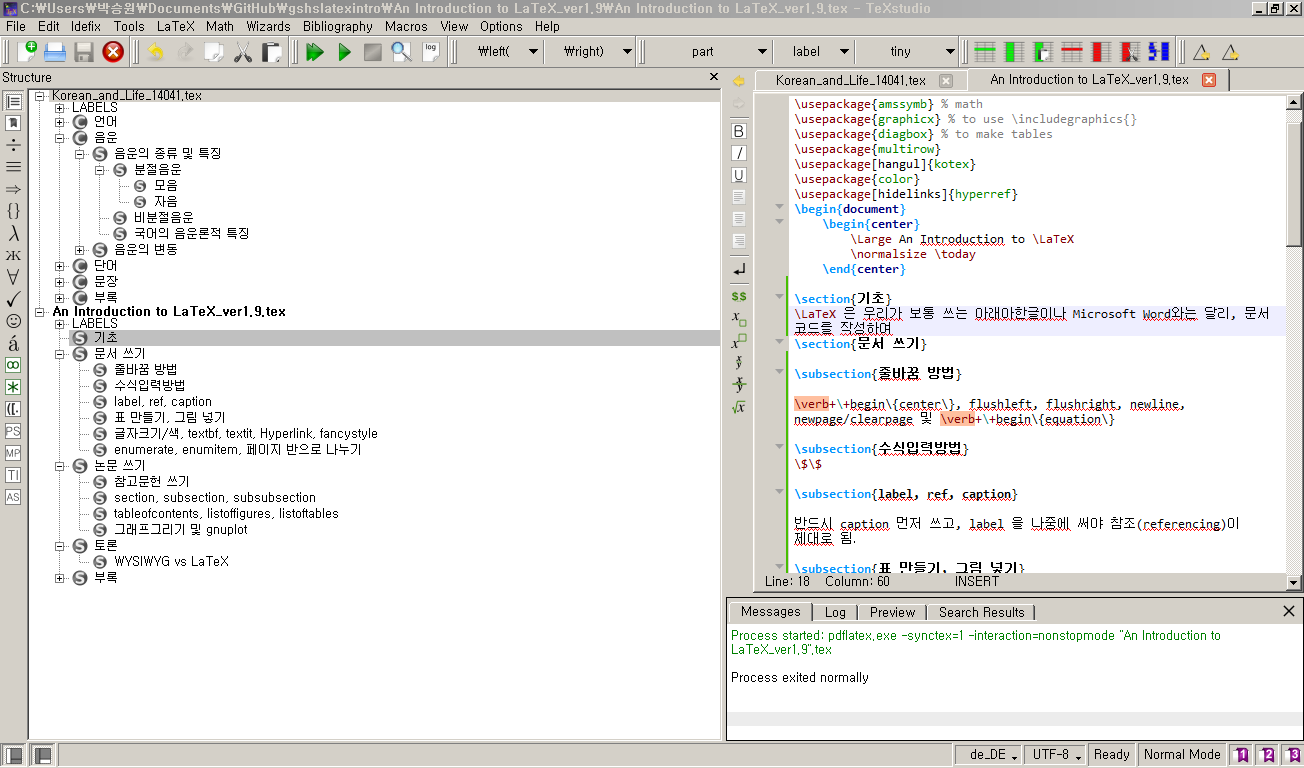
\includegraphics[width=\textwidth]{texstudio.png}
	\end{center}
	\caption{TeXstudio를 이용하여 이 문서를 편집하는 화면}
	\label{texstudio}
\end{figure}

\section{문서 작성하기}

\subsection{헤더}
\LaTeX 문서는 기본적으로 헤더 - 문서 와 같이 구성된다. 헤더는 문서의 내용이 
시작되기 전 사용할 기능을 정의하고 문서의 기본 틀을 잡는 등의 역할을 한다(즉, 
클래스·패키지 선언, 커맨드 정의/재정의 등은 헤더에서 이루어져야 한다).
헤더 예시는 다음과 같으며, 헤더 다음에는 \verb|\begin{document}|와 
같이 문서가 시작된다. (헤더 예시를 주의 깊게 읽을 필요는 없다)

모든 모드는 \verb|\begin{...}|로 시작하고 \verb|\end{...}| 로 끝난다.

\begin{verbatim}
\documentclass[11pt,a4paper]{article}
\usepackage[left=25mm,right=25mm,top=30mm,bottom=30mm]{geometry}
\usepackage{amsmath}		% math
\usepackage{amssymb}		% math
\usepackage{graphicx}		% to use \includegraphics{}
\usepackage{diagbox}		% to make advanced tables 
\usepackage{multirow}		% to make advanced tables 
\usepackage[hangul]{kotex}	% to use Korean
\usepackage{color} 		% to use color font 
\usepackage[hidelinks]{hyperref}% to insert hyperlinks
\end{verbatim}

문서의 \LaTeX\enspace 기본 양식이 있다면 헤더는 작성된 상태일 것이다. 
gshslatexintro에서는 GSHS에서 쓸 수 있는 다양한 양식을 제공하고 있다. 양식을 
사용할 경우 헤더에 대해서는 생각할 필요가 없을 것이다.

그러나 양식과 다르게 조판을 하고 싶거나, 새로운 문서를 만들어야 하는 
상황이라면 어느 정도 기본적인 지식이 필요할 것이다. 여기서는 매우 중요한 몇 
가지에 대해서만 짚고 넘어가고, 추가로 필요한 사항은 \lshort 을 읽어보기를 
바란다.

\begin{itemize}
	\item \verb|documentclass[...]{...}|
	
	대괄호 안에 글자 크기와 용지 크기 설정 등을 한다. 글자 크기는
	10pt, 11pt, 12pt를 지원하며 기본값은 10pt이다. 용지 크기는 a4paper, 
	letterpaper 등을 지원하며 기본값은 letter이다.
	
	중괄호 안에 전체적인 양식을 지정한다. article, report, book 등의 여러 
	클래스가 있으나 일반적으로는 article을 사용한다. 참고로 report는 
	박사학위 논문 급의 긴 보고서를 작성할 때 쓰인다.
	
	\item 
	\verb|\usepackage[left=...,right=...,top=...,bottom=...]{geometry}|
	
	용지의 여백을 설정하기 위한 패키지이며 일반적으로 25mm, 25mm, 30mm, 
	30mm을 사용하는 편이다(한/글의 A4 용지 기본 설정과 상당히 유사하다).
	
	\item \verb|usepackage[hangul]{kotex}|
	
	한글을 사용하기 위한 패키지이다. 대괄호 안의 hangul 옵션은 각종 영어로 
	쓰이는 단어를 한국어로(예 : figure $\rightarrow$ 그림) 바꾸어 준다.
	
	\item \verb|\usepackage{dhucs-setspace}|\\
	\verb|\SetHangulspace{...}{...}|
	
	kotex 패키지를 사용하는 경우에, 줄 간격을 설정하는 패키지이다.
	SetHangulspace의 앞 중괄호가 본문의 줄 간격이 되며, 뒤 중괄호가 표 등의 
	줄 간격이 된다. 숫자는 배수이다.(예 : 160\%를 사용하려면 1.6 입력)
\end{itemize}

\subsection{줄바꿈 방법}

본문에서 줄을 바꾸기 위해서는 기본적으로 두 번 개행하면 된다. 강제개행을 원할 
때는 \verb|\\| 를 사용한다.

\verb+\+begin\{center\}, flushleft, flushright, newline, newpage/clearpage 및 \verb+\+begin\{equation\}

\subsection{문단}
문단의 구분은 기본적으로 section, subsection, subsubsection, paragraph, 
subparagraph의 5단계로 구성되어 있다. \verb|\section{...}|과 같이 쓰면 section 
제목이 나오고, \verb|\subsubsection{...}|과 같이 쓰면 subsubsection의 제목이 
나온다. 번호는 순서에 맞게 자동으로 붙어 나온다. 참고로 subsubsection은 
documentclass가 article일 경우 숫자가 나타나지 않고 번호만 나온다. 그림 
\ref{section} 참조.

\begin{verbatim}
\section{음운의 종류 및 특정}
음운의 종류에는 `말'을 `ㅁ', `ㅏ', `ㄹ'와 같이···
\subsection{분절음운}
\subsubsection{모음}
\end{verbatim}

\begin{figure}[h]
	\begin{center}
		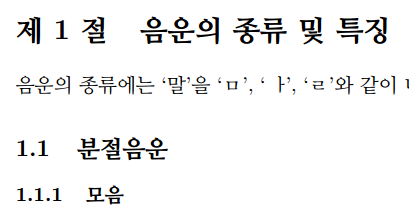
\includegraphics{section_subsection_subsubsection.png}
	\end{center}
	\caption{section, subsection, subsubsection의 예시}
	\label{section}
\end{figure}

\subsection{수식 입력 방법}
\LaTeX 의 수식은 행 내 수식과 보여주기 수식으로 나뉜다. 행 내 수식은 \verb|$|과 
\verb|$| 사이에 입력하며, 보여주기 수식은 
\verb|\begin{displaymath}|과 \verb|\end{displaymath}| 사이에 입력한다.

수식 조판은 \LaTeX 의 강력한 기능 중 하나이다. 사용법을 제대로 익히고 싶다면 
\lshort 를 먼저 읽어보는 것도 좋다.
여기서는 기본적인 몇 가지 수식 입력 방법만을 설명한다.

\begin{itemize}
	\item 위, 아래 첨자는 각각 \verb|^{...}|과 \verb|_{...}|을 이용하여 
	입력한다.
	\item 분수 표기는 \verb|\frac{분자}{분모}|로 한다.
	\item 수식 안에서 곧은 글꼴을 쓰고 싶다면 \verb|\mathrm{...}|을 
	이용한다.
	\item 수식 안에서 {\bf 한글}을 사용하고 싶다면, 반드시 
	\verb|\text{...}|를 사용하여야 한다(단, amsmath 패키지 필요). mbox나 
	text 안은 수식이 아닌 텍스트로 취급되며 따라서 
	기울임도 적용되지 않는다.
\end{itemize}

예시로 $F^{\prime}_{\text{초기}}$를 입력하고 싶다면 
\verb|$F^{\prime}_{\text{초기}}$|라고 쓰면 된다.
\begin{equation} \label{eq:example1}
	\text{속력} = \frac{\text{거리}}{\text{시간}}
\end{equation}

식 \ref{eq:example1}과 같은 표시형 수식을 입력하기 위한 코드는 다음과 같다.

\begin{verbatim}
\begin{displaymath}
	\text{속력} = \frac{\text{거리}}{\text{시간}}
\end{displaymath}
\end{verbatim}

\subsubsection{기호} \label{section_symbol}
\LaTeX 에서는 몇 가지 기호들이 명령어로 사용되기 때문에, \textbackslash 를 기호 
앞에 붙여야 제대로 표시되는 문자들이 있다. 키보드에서 입력할 수 있는 문자 중 
\textbackslash 를 필요로 하는 문자들은 다음과 같다.

\begin{verbatim}
~, $, %, ^, &, _, {, }
\end{verbatim}

\LaTeX 에서 따옴표를 입력할 때는 \verb|`|(QWERTY 키보드 기준으로 맨 왼쪽 위의 
아랫글쇠. \LaTeX 에서는 plain text에서조차 이 기호가 여는 작은따옴표로 
나온다)와 \verb|'|를 이용한다. 앞의 기호가 여는 따옴표이고, 뒤의 기호가 닫는 
따옴표이다. 두 번 연달아 입력하면 큰따옴표를 쓸 수 있다(단, 수식에서는 두 번 
써도 작은따옴표가 두 번 나온다). 예시로 ``90\% 할인!!''을 쓰려면
\verb|``90\% 할인!!''|이라고 쓰면 된다.

\LaTeX 은 기본적으로 7비트 문자열에 최적화되어 있기 때문에 유니코드 기호를 
입력할 때는 수식을 사용하여야 한다. 때문에 자판에 없는 기호를 쓰려면 대부분 
수식에서 활용해야 한다. 예를 들어, 물결표($\sim$)를 입력하려면 
\verb|$\sim$|이라고 써야 한다.

TeXstudio에서는 왼쪽의 메뉴에서 다양한 기호의 명령어들을 자동으로 입력할 수 
있게 해 준다. 사용을 원하는 기호가 있다면 수식 모드에서 기호를 눌러 사용하면 
된다. 원하는 기호를 찾지 못했다면 
\href{http://detexify.kirelabs.org/classify.html}{Detexify}에서 찾을 수도 있다.

\subsection{떠다니는 개체}
표, 그림 등은 떠다니는 개체로 위치가 고정되어 있지 않고 떠다닐 수 있기 때문에 
떠다니는 개체라고 한다.

\subsubsection{표}
\LaTeX 에서 표를 작성하는 것은 조금 까다롭다. 때문에 여기서는 사용할 수 있는 
몇 가지 방법에 대해서만 다룰 것이다. 자세한 내용은 \lshort 을 참고하는 것이 
좋다.

\paragraph{표 생성기 이용}
인터넷에 있는 \href{www.tablesgenerator.com}{LaTeX Table Generator}를 사용할 
수 있다. 원하는 표를 만든 뒤 Generate 버튼을 누르고 Copy to clipboard로 복사한 
다음 tex 파일에 붙이면 된다.

\paragraph{엑셀 매크로 이용}
\href{https://www.ctan.org/pkg/excel2latex}{CTAN}에서 제공하는 엑셀 매크로를 
다운받아 사용할 수 있다. Download를 눌러 압축 파일을 다운받은 뒤 xla 파일을 
실행시키면(매크로를 허용해야 한다) 엑셀 추가 기능 탭에 Convert table to LaTeX가 
생긴다. 표를 만든 뒤 범위 지정 후 Convert table to LaTeX 버튼을 누르고(역시 
매크로 허용 필요) Copy to clipboard하면 표의 내용이 복사된다. 셀의 정렬은 미리 
왼쪽, 가운데, 오른쪽 중 하나를 지정해주어야 하며(지정하지 않으면 어떻게 
변환될지 모른다), 주의할 점은 이 매크로는 테두리까지 복사하지는 않는다.
이 방법을 쓸 때는 헤더 부분(\verb|\begin{document}| 이전 부분)에 다음의 코드를 
작성하여야 toprule, midrule, bottomrule에 의한 에러가 발생하지 않는다.
\begin{verbatim}
\makeatletter
\newcommand{\thickhline}{%
	\noalign {\ifnum 0=`}\fi \hrule height 0.5mm
	\futurelet \reserved@a \@xhline
}
\makeatother
\newcommand{\toprule}{\thickhline}
\newcommand{\midrule}{\hline\hline}
\newcommand{\bottomrule}{\thickhline}
\end{verbatim}
작은따옴표는 QWERTY 키보드 맨 왼쪽 위 키의 아랫글쇠이다. 복잡하게 따라 칠 필요 
없이, 이 문서의 tex 파일에서 복사하면 된다.

\subsubsection{그림} \label{figuresec}
그림을 넣을 때 기본적으로 사용하는 구조는 다음과 같다.
\begin{verbatim}
\begin{figure}[...]
	\begin{center}
		\includegraphics[...]{...}
	\end{center}
	\caption{...}
	\label{...}
\end{figure}
\end{verbatim}

맨 뒤 대괄호는 떠다니는 개체의 위치를 지정한다. 바로 그 자리에 넣고 싶으면 h, 
쪽의 맨 위는 t, 아래는 b, 떠다니는 개체만 모여 있는 쪽을 만들어 넣고 싶으면 p를 
쓴다. 여러 개를 같이 쓰면 그 중 제일 어울리는 위치에 삽입된다. 이는 표의 위치를 
지정할 때에도 동일하다.

includegraphics 뒤의 대괄호는 그림의 크기나 회전 방향을 결정한다. scale=...은 
원본 크기의 몇 배로 크기를 지정한다. width=...은 너비 지정, height=...은 높이 
지정이다. width나 height 옵션 중 하나만 쓰면 나머지 하나는 비례하여 늘어나거나 
줄어든다(둘 다 지정하면 원본 비율과 다르게 된다).

includegraphics 뒤의 중괄호에는 그림 파일 이름을 쓴다. 파일은 tex 파일과 같은 
폴더(디렉토리)에 있으면 된다.
지원하는 형식은 기본적으로 eps 파일이며 jpg, png, pdf 파일 등을 지원한다.
주의해야 할 점은 파일 이름에는 공백이 없어야 한다는 점이다.

\paragraph{Excel 그래프}
그래프를 그리면 TeX에 넣을 수 있도록 쉽게 변환해주는 프로그램들이 있지만, 
대부분은 Microsoft Office Excel을 이용하여 데이터 처리를 한 뒤 그래프를 그릴 
것이다. 이 경우 그래프를 비트맵 이미지가 아닌 벡터 형태로 넣을 수 있는 방법은 
pdf로 저장한 뒤 삽입하는 것이다.
하지만 그냥 pdf로 저장하면 원본 크기가 맞지 않을 뿐더러 여백도 생긴다. 따라서 
다음의 방법을 사용하는 것이 좋을 것이다.

\begin{shadequote}{일화실 보고서 작성 도움말}
	Excel에서 그래프를 그린 뒤 원본 크기로 pdf로 저장하는 방법은
	다음과 같습니다.
	
	먼저 Excel에서 그래프의 크기를 차트 도구-서식-크기를 통해
	확인 또는 지정한 뒤, 그래프를 복사합니다.
	다음으로 Powerpoint에서 디자인-페이지 설정에 들어가 슬라이드 크기를
	그래프와 같은 크기로 지정하고, 붙여넣기합니다.
	이렇게 하면 그래프가 슬라이드에 정확히 맞게 차게 됩니다.
	맞지 않는다면 크기가 잘못된 것입니다.
	그 다음 파일-다른 이름으로 저장-PDF 또는 XPS를 선택한 다음
	저장하시면 됩니다.
	
	게시 옵션으로 ISO 19005-1 호환을 권장하나 하지 않으셔도 문제 없습니다.
%	Office 2007 기준으로 설명해서, 확인하는 경로가 다를 수 있기는 
%	합니다.
	includegraphics 옵션에서 scale=1로 지정하면 원본 크기가 됩니다.
\end{shadequote}

\paragraph{일러스트나 그래프를 넣는 기타 방법들}
보고서를 작성하다 보면, 확대해도 깨지지 않는 벡터 형식의 그래픽으로 
일러스트를 해야 할 때가 생긴다. 이럴 때, 아래의 방법들이 실제 현장(대학원?)
에서 사용되는 것들이라고 한다. 
특히, 필자의 경험에 의하면, GeoGebra를 이용하여 원하는 도형을 그리면 화면 안에
있는 부분을 캡처하듯이 tikz code 로 내보내 주기 때문에 매우 편리하다. 
또한, GeoGebra는 오픈소스 프리웨어이므로 학생이 사용하기 좋다.
\begin{itemize}
\item 	Origin
\item 	ggplot
\item 	matplotlib
\item 	gnuplot
\item 	Adobe Illustrator
\item 	tikz
\item 	GeoGebra : Export to tikz
\end{itemize}

\subsubsection{캡션}
떠다니는 개체에는 캡션을 달 수 있다. 개체 내에 \verb|\caption{...}|을 쓰고 
중괄호 안에 캡션의 내용을 넣는다. 번호는 문단 번호와 같이 자동으로 달린다.

\subsection{레이블과 참조}
레이블은 개체나 문단, 수식 등의 번호를 참조할 때 쓰인다. 예를 들어 개체에
\verb|\label{asdf}|라고 달았다면, 다른 곳에서 그 개체의 번호를 불러오고 싶으면
\verb|\ref{asdf}|라고 쓰면 된다.
개체에 레이블을 달 때는 개체 내에 달면 되고, 문단에 달 때는 문단 제목 뒤에 달면 
된다.

주의할 점은 떠다니는 개체에서 label을 할 때에는 반드시 caption 먼저 쓰고, label 
을 나중에 써야 참조가 제대로 된다는 점이다.

\subsubsection{자동 조사 기능}
참조를 할 때 번호에 따라 붙어야 하는 조사가 달라지는 경우가 있다. (예 : 그림 
2가 / 그림 3이) 이러한 경우 둘 중 아무 조사나 쓰고 앞에 \textbackslash 를 붙여 
주면 번호에 따라 알아서 조사를 붙인다.

\section{논문 쓰기}

\subsection{참고문헌 쓰기}
참고문헌은 thebibliography를 이용하여 쓰며 맨 마지막에 참고 문헌이 추가된다. 
이 문서에 쓰인 참고 문헌을 입력하기 위한 코드의 형태는 다음과 같다.
\begin{verbatim}
\begin\{thebibliography\}\{00\}
\bibitem{gshs}{http://gs.hs.kr}
\bibitem{sjgshs}{https://student.gs.hs.kr}
\end\{thebibliography\}
\end{verbatim}
\verb|\cite{...}| 와 같이 쓰면 참고문헌의 논문 번호가 나온다. 예를 들어
\verb|\cite{sjgshs}|라고 하면 \cite{sjgshs}\이 출력된다.


\subsection{차례}
\LaTeX 은 차례도 자동으로 만들어준다. 다음의 함수를 문서 내에 넣으면 차례가 
출력된다.

\begin{verbatim}
\tableofcontents : 목차(Table of Contents)	
\listoffigures : 그림 차례(List of Figures)
\lisfoftables : 표 차례(LIst of Tables)
\end{verbatim}




\section{토론}
이 단락에 한하여 다중 관점이 허용된다. 자유로운 의견 추가가 가능하다.

\subsection{WYSIWYG vs LaTeX}
WYSIWYG는 What you see is What you get의 약자로 출력물을 보면서 작업하는 
방식이고, LaTeX은 컴파일을 통해 조판하는 방식이다.

LaTeX은 적은 노력으로 미려한 조판 결과를 얻을 수 있고, 양식이 정해져 있다면 
내용을 채워 넣기만 하면 될 뿐이므로 빠른 작업 속도를 얻을 수 있다.
그러나, 딱히 문서의 조판이 중요하지 않을 때는 반드시 LaTeX을 사용하지 않아도 
되며, 특히 시간이 없는데 주어진 양식 파일마저 없다면 개인적으로 LaTeX으로 
작성하는 것을 권하지 않는다. LaTeX은 편하지만 반드시 빠르지는 않다. -익명의 
편집자

우리가 흔히 사용하는 워드프로세서는 Microsoft Word, 아래아한글 한글과컴퓨터,
 그리고 \LaTeX 이 있다. \LaTeX 을 사용할지의 여부는 
\section{부록}

\clearpage
\subsection{Quick Table}
WYSIWYG 방식의 워드프로세서에서 \LaTeX 을 사용하기 시작할 때, 이 표를 따로 출력하여 들고 다닌다면 빠르게 적응할 수 있을 것이다.

\begin{table}[h]
	\centering
	\begin{tabular}{|c|l|}
		\hline
		한글 & \verb+\+usepackage[hangul]\{kotex\} 가 헤더에 반드시 있어야 함.\\
		\hline
		italic & \verb+\+textit\{...\} 또는 \{\verb+\+it ... \} \\
		\hline
		bold & \verb+\+textbf\{...\} 또는 \{\verb+\+bf ...\} \\
		\hline
		취소선 & \verb+\+sout\{...\} \\
		\hline
		밑줄 & \verb+\+underline\{...\} \\
		\hline
		개행 & 문서 상에서의 두번 개행, 혹은 \verb+\+\verb+\+ , 혹은 \verb+\+newline \\
		\hline
		페이지 넘김 & \verb+\+clearpage \\
		\hline
		따옴표 & \ref{section_symbol} 절 참조 \\
		\hline
		\%, \&, \_, \{, \} & 각각 \verb+\+\%, \verb+\+\&, \verb+\+\_, \verb+\+\{, \verb+\+\} \\
		\hline
		\~{} & 쓰지 말자. \\
		\hline
		좌측정렬 & \verb+\+begin\{flushleft\} ... \verb+\+end\{flushleft\} 또는 \{\verb+\+flushleft ...\}.\\
		\hline
		우측정렬 & \verb+\+begin\{flushright\} ... \verb+\+end\{flushright\} 또는 \{\verb+\+flushright ...\}.\\
		\hline
		중앙정렬 & \verb+\+begin\{center\} ... \verb+\+end\{center\} \\
		\hline
		폰트크기 & 표 아래의 글 참조 \\
		\hline
		폰트 & (고급) \\
		\hline
		폰트 색 & \verb+\+usepackage\{color\} \\
		\hline
		각주 & \verb+\+footnote\{...\} \\
		\hline
		용지크기 & a4paper 등등. 고급기능이므로 생략. \\
		\hline
		편집용지 & (고급 기능) \\
		\hline
		머리말/꼬리말 & \verb+\+usepackage\{fancyhdr\}를 헤더에 넣어준 후 \verb+\+chead\{\} \verb+\+cfoot\{\} \\
		\hline
		페이지 절반 분할 & \verb+\+usepackage\{multicol\},  \verb+\+begin\{multicols\}\{2\} ... \verb+\+end\{multicols\} \\
		\hline
		줄간격 조정 & \verb+\+linewidth[...] \\
		\hline
		들여쓰기 조정 & \verb+\+usepackage\{indentfirst\} 등 \\
		\hline
	\end{tabular}
	\caption{Quick conversion table}
	\label{Quick_table}
\end{table}
{\tiny \verb+\+tiny} {\scriptsize \verb+\+scriptsize} {\footnotesize \verb+\+footnotesize} {\small \verb+\+small} {\normalsize \verb+\+normalsize} {\large \verb+\+large} {\Large \verb+\+Large} {\LARGE \verb+\+LARGE} {\huge \verb+\+huge} {\Huge \verb+\+Huge}
\end{document}

\tableofcontents
\listoffigures
\listoftables

\begin{thebibliography}{00}
\bibitem{gshs}{http://gs.hs.kr}
\bibitem{sjgshs}{https://student.gs.hs.kr}
\end{thebibliography}


\end{document}
